%% Ezen fájl tartalma csupán csak jegyzet még, pontosításra szorul benne sok dolog még... %%

\Chapter{GAN}
A \textit{Generative Adverserial Network} (GAN), egy olyan generatív modell, amely nem a megszokott statisztikai alapokon optimalizál, mint például az Autoencoder vagy pixelRNN modellek, hanem játékelméleti megközelítést alkalmaz. (Az generatív modellekről lehetne írni esetleg egy áttekintést, hogy miért éppen a GAN-ra esett a választás mondjuk a VAE-val szemben?)
A tanulás során két neurális hálózat versenyzik egymással: egy \textit{generátor}, amelynek az a szerepe, hogy a tanítómintákhoz hasonló adatot generáljon a bemeneti zajból és egy \textit{diszkriminátor}, amely egy bináris osztályozó, amely a generátor által generált adatot vizsgálja és eldönti, hogy az valódi vagy hamis.
A tanítás során ezen két háló versenyzik egymással, együtt fejlődve.
A generátor bemenete egy zajvektor, amely általában Gauss- vagy egyenletes eloszlásból állítunk elő. Ezt a zajvektort az irodalom látens térnek is nevezi, hiszen a tanítás során a modell megtanulja, hogy ezen többdimenziós tér egyes pontjaira milyen kimenetet generáljon. Vagyis ezzel lényegében kitölti a rendelkezésre álló tér tartományait a megtanult jellegzetességekkel. A generátorral ezen tér bármely pontját mintavételezve a tanítóhalmazhoz hasonló adatokat generálhatunk.

\Section{Adathalmaz, tanítóhalmaz előkészítése}
A tanításhoz szükségünk van egy megfelelő adathalmazra. Képek generálásához legegyszerűbb esetben elegendő lehet képek rendezetlen halmaza is és a modellre bízhatjuk, hogy ismerje fel az egyes osztályok jellegzetességeit. Megfelelő regularizációs technikákkal igazán változatos képek generálására lesz képes a betanított modell.

Ha az adathalmaz rendelkezik osztályokkal is, úgy az osztály-címkéket is felhasználhatjuk a GAN hálózatunk tanításához. Így egy plusz bemenet segítségével könnyebben tudunk majd megfelelő képeket előállítani. (Ezt a technikát class-conditioningnak nevezik, de utána kell nézzek)

Egyes adathalmazokhoz igen részletes annotációkat is mellékelnek. A képeken megfigyelhető objektumokat határoló dobozokkal, vagy pixel szinten is jelölik. Így igen részletes információkat kínálnak a kép tartalmáról. Egy igazán hasznos annotációk lehetnek a természetes nyelvű leíró mondatok is, amelyekből általában többet is mellékelnek egy-egy képhez.

Ha kiválasztottuk a modellünkhöz megfelelő adathalmazt, akkor a probléma és a modell bonyolultságától függően elő kell készítenünk az adatokat a tanításhoz.
A GAN esetében a hálózat paraméterei közé tartozik a minibatch elemszáma is. Minibatch alatt a tanítóhalmaz egy bizonyos elemszámú mintát tartalmazó szeletét értjük. A minibatch-ok alkalmazása azért lényeges, hogy egy tanítási lépés során a modell ne lássa a teljes tanítóhalmazt. A hálózat tanításához általában sok mintára van szükségünk, így egy darabban való tanítás igen nehézkes és számításigényes lenne. De nem csupán ez jelenti a fő veszélyt, Ha egy lépésben láthatná a diszkriminátor az összes képet, akkor túlságosan is megnőne a teljesítménye és a generátornak esélye sem lenne felzárkózni. A minibatch-okon való tanítás tehát elengedhetetlen része a tanítási folyamatnak és a megfelelő ütemű tanulás biztosításának.

\Section{Modell tanítása}
Ha a legegyszerűbb esetet vizsgáljuk és csak a képek rendezetlen halmazára tanítjuk a modellt, mindenféle kiegészítő információ és annotáció nélkül, akkor a tanítás a következőképpen zajlik.
A továbbiakban a következő jelöléseket használom: legyen $D$ a \textit{diszkriminátor}, $G$ pedig a \textit{generátor}.

\SubSection{Hibafüggvények}
A $G$ és $D$ hibájának számolása a bináris kereszt-entrópián alapszik.
A bináris kereszt-entrópia hibafüggvény a következőképpen írható fel:
$$L(\hat y, y) = y . \log \hat y + (1-y). \log (1 - \hat y)$$
Ahol $\hat y$ a predikció, $y$ pedig a valós címke

\noindent \textbf{Diszkriminátor hibafüggvénye}\\
A $G$ generátor egy $z \in \mathbb{R}^n, n \geq 1$ bemeneti zajvektor alapján előállít egy generált adatot $G(z)$.
A $D$ diszkriminátor egy bináris osztályozó, amelynek feladata, hogy az $x$ és $G(z)$ bemeneteit osztályozza.\\
$D(x)$ esetén 1, $D(G(z))$ esetén pedig 0 címkét várunk.\\
A hibafüggvény számolása két lépésben történik a kétféle bemenet miatt:

$D(x)$-re nézve a kereszt-entrópia a következő:
$$L(D(x), 1) = 1.\log D(x) + (1 - 1).\log(1 - D(x))$$
$$L(D(x), 1) = \log D(x)$$
Vagyis jelen esetben $D$-nek a $\log(D(x))$-et kell maximalizálnia.

$D(G(z))$-re nézve a kereszt-entrópia a következő:
$$L(D(G(z)), 0) = 0.\log D(G(z)) + (1 - 0).\log(1 - D(G(z)))$$
$$L(D(G(z)), 0) = \log(1- D(G(z)))$$
Vagyis a $\log(1 - D(G(z)))$-t kell maximalizálnia.

Egyetlen mintára a hibafüggvény a következőképpen néz ki:
$$\max V(D) = \log D(x) + \log(1 - D(G(z))$$

Batch-ra nézve:
$$\max V(D) = \mathbb{E}_{x \sim P(x))} \left[\log D(x) \right] + \mathbb{E}_{z \sim P(z))} \left[\log(1 - D(G(z))) \right]$$

Ahol a $P(x)$ a valószínűségi eloszlása a tanítóhalmaznak, $P(z)$ a valószínűségi eloszlása a $z$ zajvektornak. (látens tér).

\noindent \textbf{Generátor hibafüggvénye}\\
A $G$ generátor feladata az, hogy megtévessze a $D$ diszkriminátort azáltal, hogy a tanítóhalmazhoz hasonló adatokat generáljon.
Vagyis a $G$ érdeke az, hogy a $D(G(z))$ 1-es címkét kapjon 0 helyett.

Tehát a bináris keresztentrópia egy mintára:
$$L(D(G(z)), 0) = \log(1 - D(G(z))$$
$D$ minimalizálni kívánja a $D(G(z))$-t, míg a $G$ maximalizálni szándékozik azt.

A $G$ a tanítás során sosem fog valódi adatot látni, de a teljesség kedvééert a hibafüggvénye a következőképpen írható fel (Csak a második kifejezést minimalizálja valójában):
$$\min V(G) = \mathbb{E}_{x \sim P(x))} \left[\log D(x) \right] + \mathbb{E}_{z \sim P(z))} \left[\log(1 - D(G(z))) \right]$$

Vagyis a GAN hálózat tanítása során $D$ és $G$ egy minimax játékot játszanak a $V(G, D)$ értékfüggvénnyel.
$$\min_{G}\max_{D}V(D, G) =  \mathbb{E}_{x \sim P(x))} \left[\log D(x) \right] + \mathbb{E}_{z \sim P(z))} \left[\log(1 - D(G(z))) \right]$$

\SubSection{Optimalizáló módszer}
A Generátorban is és a Diszkriminátoban is az Adam optimalizáló használatos. (Kezdeti paraméterek, learning rate, beta1-2)
Itt vagy egy másik kis fejezetben be lehetne mutatni az optimalizáló módszereket?

\SubSection{Tanítási lépés}
%% GAN 2014 cikkből

A GAN hálózat egy tanítási lépése a következő lépésekből áll:

Legyen $m$ a minibatch elemszáma $m \in \mathbb{N}$

\begin{enumerate}
	\item Hozzunk létre $m$ darab zajmintát $(z_1, \ldots, z_m)$ gauss eloszlásból $P_g(z)$.
	\item A tanítóhalmazból emeljük ki a soronkövetkező $m$ darab tanítómintát (képet), és ezt jelöljük $(x_1, \ldots, x_m)$-el $P_{\text{data}}(x)$
	\item Frissítsük a $D$ diszkriminátort a sztochasztikus gradiens emelkedésével (?? tükörfordítás)
$$ \nabla \theta_d \frac{1}{m} \sum_{i=1}^{m} \left[\log D(x_i) + \log(1 - D(G(z_i))) \right]$$
	\item Frissítsük a $G$ generátort a sztochasztikus gradiens lejtésével (?? tükörfordítás)
$$ \nabla \theta_d \frac{1}{m} \sum_{i=1}^{m} \log(1 - D(G(z_i)))$$
\end{enumerate}
Természetesen nem egyszerre tanítjuk a GAN részeit. Az eredeti cikkben is javaslatot tesznek arra, hogy a $D$-t esetleg több lépésben is lehetne tanítani, majd a $G$-t egyetlen lépésben frissíteni.
Különböző tanítási stratégiákban ez is egy szabad paraméter lehet. Számomra megfelelő volt az 1:1-es tanítási lépés alkalmazása is... (Esetleg lehetne mérni valahogy, hogy van-e számottevő különbség...)
A tanítás hossza természetesen függ az adathalmaztól és annak méretétől, a minibatch mérettől, a modellben található paraméterektől és az optimalizáló függvénytől.

\Section{Mode-Collapse jelensége}
A mode-collapse jelenség akkor figyelhető meg, amikor a Generátor a látens tér bármely pontjára egyetlen egy (vagy ritkán kétféle) képet generál, ezzel minimalizálva a hibafüggvényét.
Egyes cikkekben az összeomlásig tanítják a felvázolt modelleket és az összeomlás előtti állapotokra állítják vissza a hálózat súlyait a használathoz (BigGAN csinált ilyet, meg még más is, de meg kell keresnem.). Az mode collepse elkerülésére és a hálózat kiegészítésére igen hasznos javaslatok jelentek meg. Ezeket külön-külön is kifejtem... (!)

\Section{Regularizációs módszerek}
(Még csak a Batch Normalization-t próbáltam az alapokon kívül)

A GAN tanítása során nehézségekbe ütközhetünk. Legrosszabb esetben nem is kezd el konvergálni a generátor kimenete a tanítóminta képeihez, viszont abban az esetben gyanakodhatunk, hogy a modellünk nem lett helyesen felépítve. Amennyiben mégis elkezd fejlődni a modell és nem csak zaj jelenik meg a kimeneten az egyes tanítólépések után, de bizonyos számú epoch után mode collapse lép fel, úgy fontolóra vehetjük a következő regularizációs technikákat.

\SubSection{Megfelelő inicializációs stratégia}

\SubSection{Ativációs függvények és  paramétereiknek a helyes megválasztása}

\SubSection{Batch normalization}

\SubSection{Spectral Normalization}

\SubSection{Experience replay}

\SubSection{Mini-batch discrimination}

\Section{Teljesítmény mérési technikák}
- Inception Score (salimans2016improved, barratt2018note)
- Fréchet Inception Distance (heusel2017gans)

\Section{Data augmentation - tanítás kevés adattal}
- karras2020training
- noguchi2019image

\Chapter{Deep Convolutional GAN példa}
Ezen architektúra természetesen a mai eredmények mellett egyszerűnek tűnhet elsőre, viszont a későbbi, fejlettebb architektúrákban többségében megfigyelhető, hogy erre építkeztek. Természetesen az architektúra egy igen egyszerű kiegészítést kínált az eredeti GAN hálózatra: konvolúciós rétegeket alkalmaz a rejtett rétegekben mind a Generátor, mind a Diszkriminátor esetében. A konvolúciós rétegek segítségével a képeken lévő összefüggő pixelek kapcsolatairól pontosabb reprezentációt kaphatunk, így képek generálásához is hasznos lehet a módszer. 

\Section{Generátor}
Az osztályozáshoz használt konvolúciós hálókkal ellentétben a Generátorban a kisebb felbontás felől haladunk a nagyobb felbontásig.
A generátor modellem első implementációjában \textit{Dekonvolúciós} rétegeket alkalmaztam, amelyet \textit{Transzponált konvolúciós} rétegnek is nevezhetünk. A Dekonvolúciós rétegek segítségével minden rejtett réteg kimenete egy nagyobb felbontású kép lesz, ellentétben a konvolúció működésével. Tehát a hálónak jelen esetben meg kell tanulnia a rétegekben az optimális felbontás-növelést. Előre megadott paraméterek a filterek darabszáma, a kernel mérete, a strides(?) és a padding. Ha a padding-ot "same"-re és ha a strides paramétert 2x2-esnek választjuk, úgy a réteg kimenetén megjelenő kép felbontása kétszerese lesz a bemeneti oldalon megfigyelhető képnek. A rejtett rétegekben kezdetben ReLU aktivációs függvényt használtam, a neuronok kezdő értékeit a He inicializációs technikával állítottam be (Hands on könyv ajánlása alapján).

\begin{figure}[h]
\centering
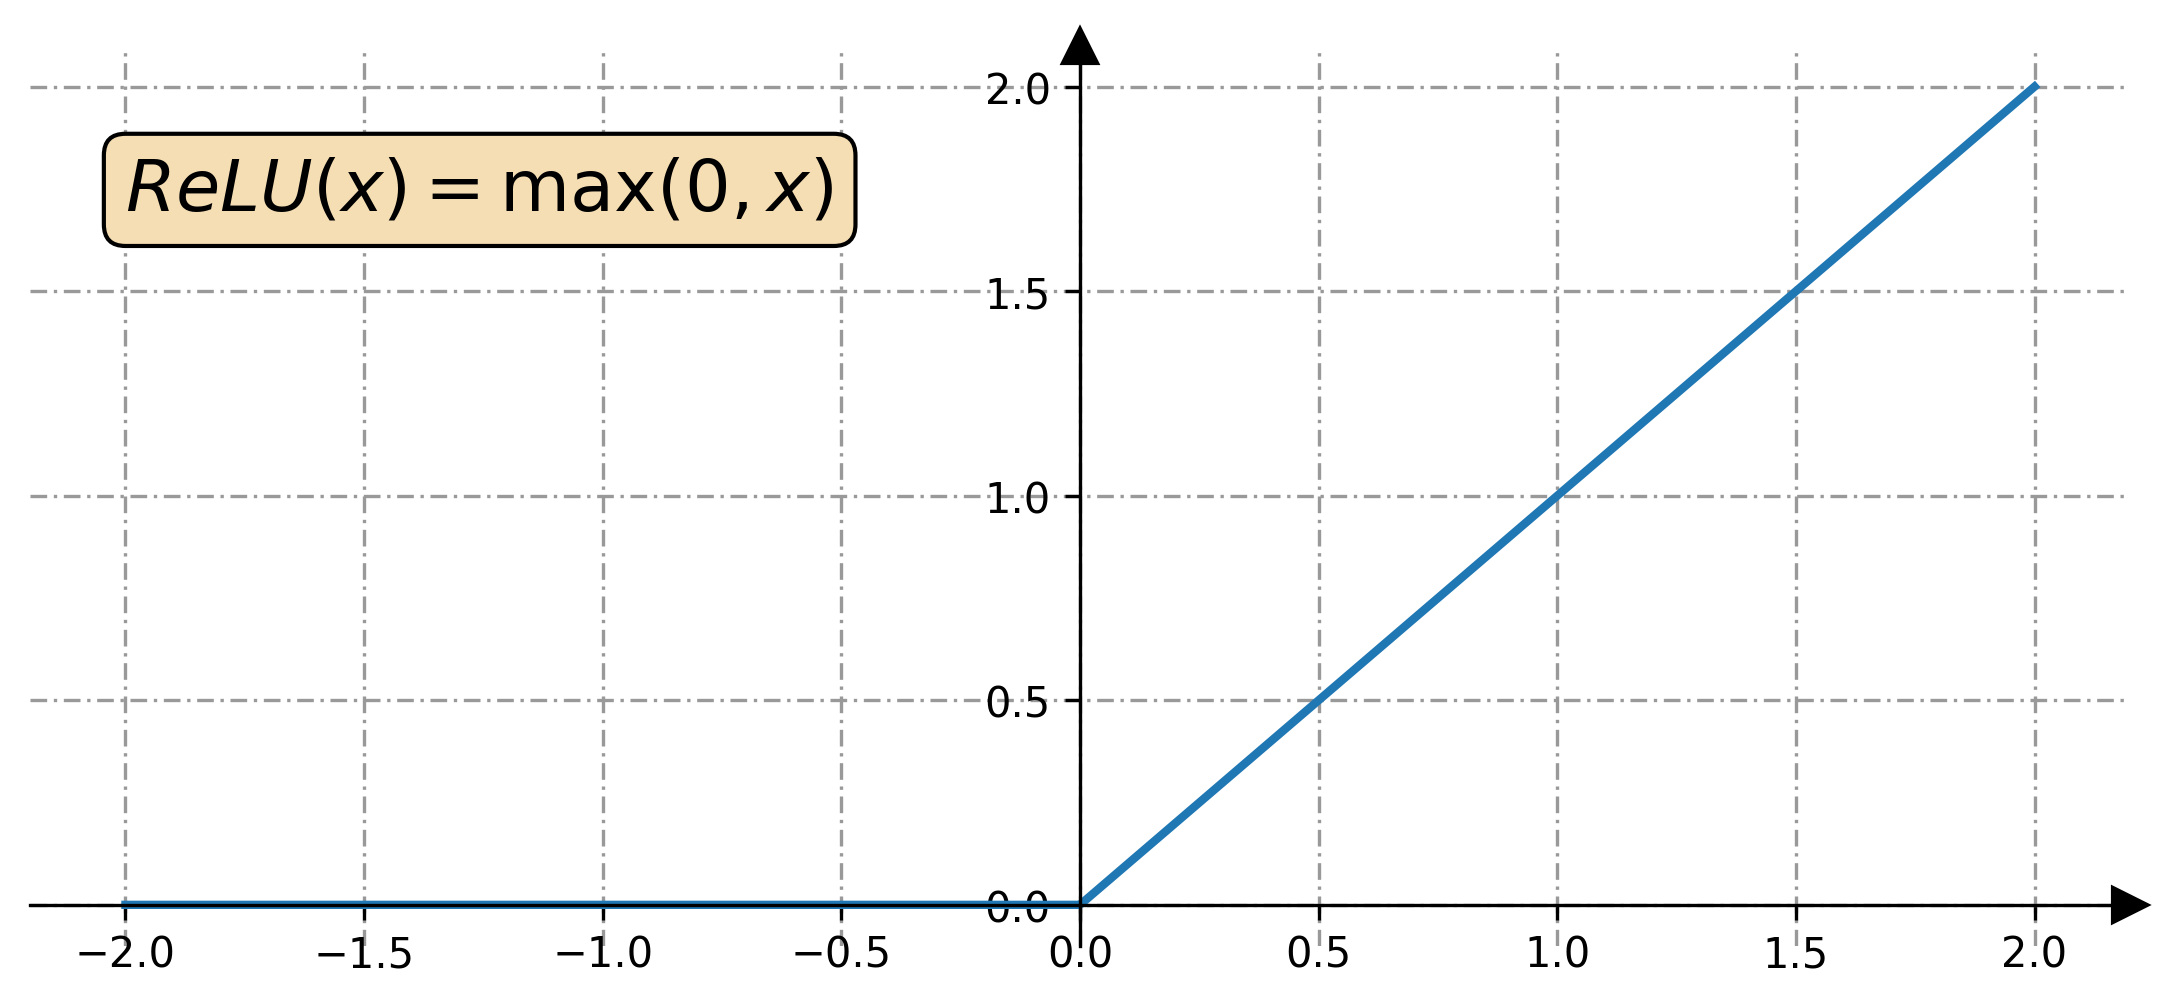
\includegraphics[width=12cm]{images/relu.png}
\caption{ReLU aktivációs függvény}
\label{fig:relu}
\end{figure}

A tanításhoz célszerű a kép pixeleinek intenzitását normalizálni a [-1, 1] intervallumra. A Generátor is ebben az intervallumban fogja a képek pixeleit generálni a hiperbolikus tanges kimeneti aktivációs függvényéből adódóan. (tanh indoklás, sigmoid helyett..) A megjelenítéshez később természetesen denormalizálnunk kell a generált képek pixelértékeit a [0, 255] tartományra.

A Generátor modell bemenetként az előre definiált látens tér dimenziójával megegyező dimenziójú zajt kap. Majd ezen bemeneti zaj segítségével állítja össze a megfelelő kimeneti képet. A tanulás során tehát a látens tér tartományaihoz rendeli a tanult jellegzetességeket és a látens teret mintavételezve dekódolható a Generátor segítségével a ponthoz tartozó kép.

A bemeneti zaj egy Reshape rétegen megy keresztül, amelyben a látens tér dimenziószámát átformázza egy 1x1xLdim dimenziójú mátrixá. Ezen réteg kimenetével a későbbi dekonvolúciós rétegek már tudnak dolgozni.
Ezután az első dekonvolúciós rétegen megy át a kapott mátrix, amely 512 darab filtert tartalmaz, 4x4-es kernelméretekkle dolgozik és 'valid' paddingot használ. Az aktivációs függvénye ReLU a már említett He inicializálással. Ezen lépés arra szolgál, hogy a látens térből előállítson egy 4x4x512-es tensort, amely az első, legkisebb felbontású képünknek tekinthetjük ebben az esetben, ahol a színcsatornák száma 512 és a felbontása 4x4.

A Generátorban ezután 2x2-es stride értékeket használva a kívánt felbontásig dekonvolúciós rétegeken keresztül növekszik a felbontás. A kernel méretét a rétegekben egységesen 4x4-ra állítottam be, a paddig 'same' és a strides a már említett 2x2-es. Az aktivációs függvény szintén ReLU. A rétegekben haladva a filterek darabszáma pedig feleződik. A filterek optimális számára csupán csak empirikus eredményeket találtam. Az utolsó dekonvolúciós réteg 3 darab filterrel rendelkezik.

A kimeneti képnek olyan tulajdonságokkal kell rendelkeznie, mint a tanítómintában szeplő képeknek. Például ha a tanítóminta színes képekből áll, rgb színkeveréssel, vagyis három színcsatornával, úgy a Generátor kimenetén is ilyen képekre van szükségünk. Mivel az említett dekonvolúciós rétegek több mint 3 színcsatornával dolgoztak, a megjeleníthetőség miatt szükséges tehát az utolsó dekonvolúciós rétegben a 3 darab filter.
Végül a hiperbolikus tangens aktivációs függvény hatására az eredményeket a [-1, 1] intervallumba transzformálja.

\begin{figure}[h]
\centering
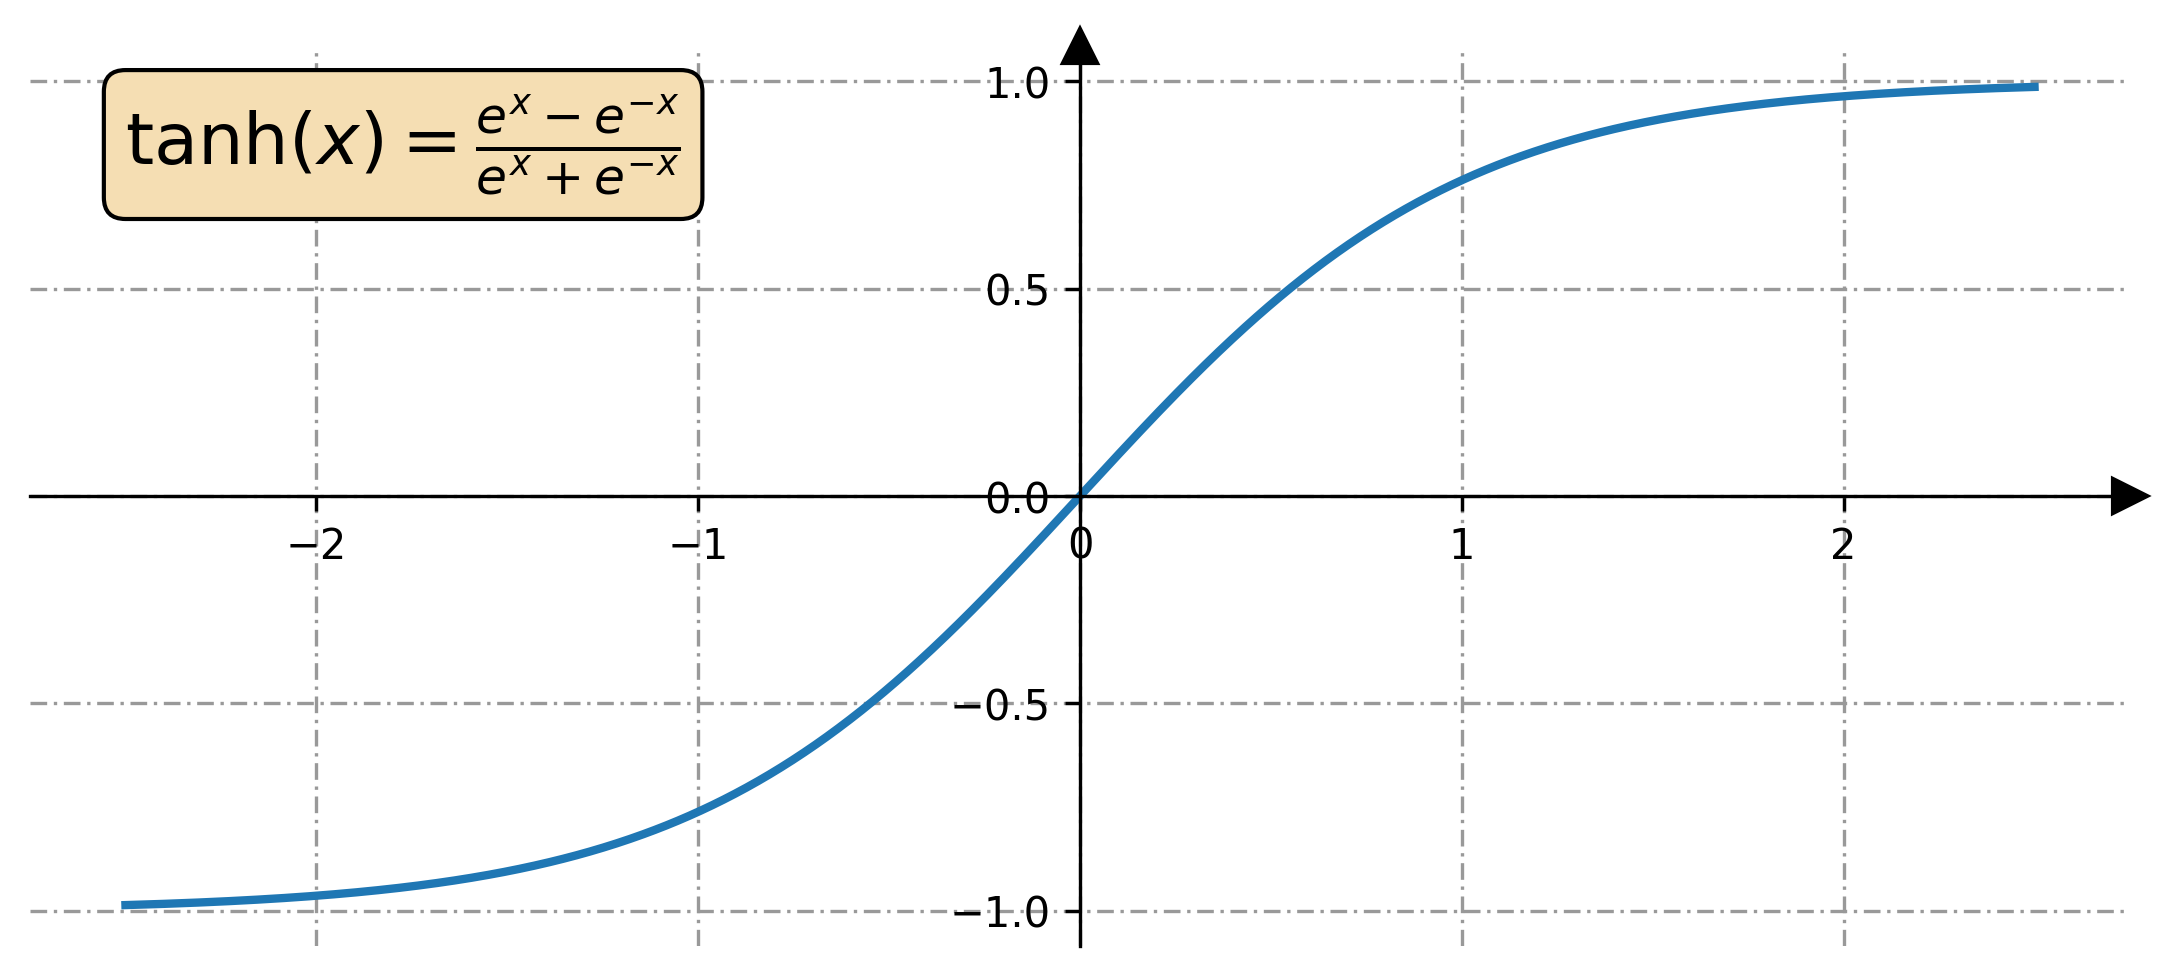
\includegraphics[width=12cm]{images/tanh.png}
\caption{Hiperbolikus tangens aktivációs függvény}
\label{fig:tanh}
\end{figure}

\Section{Diszkriminátor}

A Diszkriminátor modell lényegében egy bináris osztályozó, amely eldönti, hogy a bemenetül kapott kép valódi vagy hamis. A bemeneti kép konvolúciós rétegeken megy végig, majd a kimeneti rétegen sigmoid aktivációs függvény segítségével hozza meg a döntést. A konvolúciós rétegek segítségével a modell fel tudja tárni a képeken található jellegzetességeket. A képen található mintázatokat filterek segítségével tanulja meg, amelyek megadott kernelméretekben pásztázzák végig a bemenetet. Így az egyes konvolúciósrétegek kimeneteként egy olyan reprezentáció jön létre a bemeneti képről, amelyben érvényesülnek a pixeleket körülölelő további pixelek kapcsolatai is. Ezáltal a kimeneti aktivációs függvény előtti réteg, a szerializáció (Flattening) kevésbé fogja a kép tartalmára vonatkozó információt rontani. Mivel a tanítóminta képeinek pixelértékeit normalizáltuk a [-1, 1] intervallumra, így a diszkriminátor a bemenetén is ilyen tulajdonságú képeket vár. A Diszkriminátor felépítésben hasonlít a Generátorhoz, lényegében annak tükörképeként képzelhetjük el. Viszont a dekonvolúciós rétegek helyett konvolúciós rétegeket alkalmazunk benne.

Lényeges leírni részletesen, hogy hogy épül fel?

\Section{Problémák}

\begin{figure}[h]
\centering
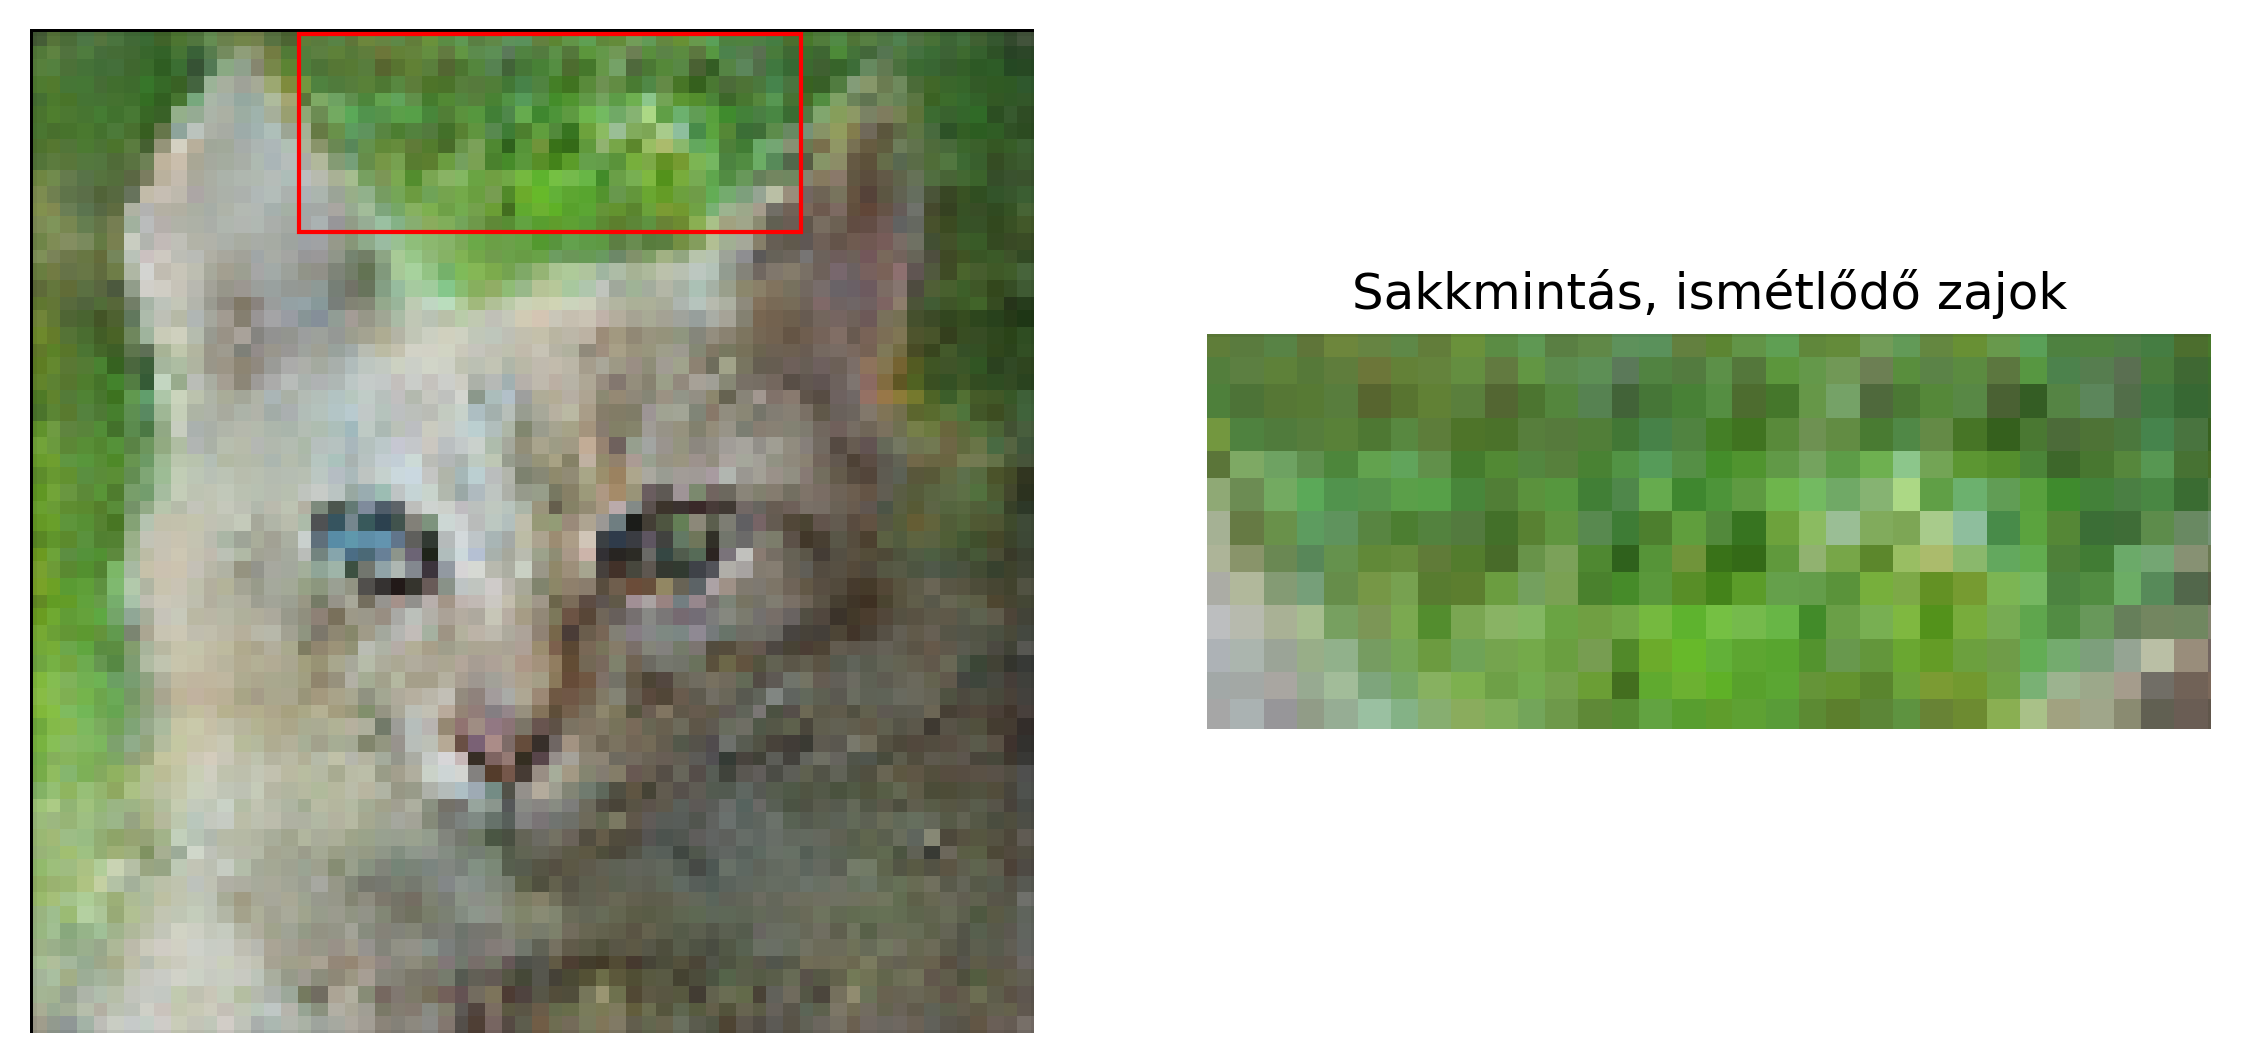
\includegraphics[width=13cm]{images/chessboard-patterns.png}
\caption{A felvázolt modell 64x64-es kimenetére egy példa - az AFHQ adathalmazon tanítva}
\label{fig:chessboard}
\end{figure}

A modell természetesen bővíthető tetszőlegesen nagy felbontásig, a felbontást növelő rétegek számával. Viszont az architektúrával problémák léphetnek fel:
\begin{itemize}
	\item A modell ebben a formájában igen hajlamos az mode collapse-re, vagyis a tanulás során jelentkező összeomlásra.
	\item A konvolúciós rétegek működéséből adódóan csupán lokális pixel-környezetekre képes összefüggő részeket generálni a modell.
	Ez a működés alacsony felbontás mellett is anomáliákat idézhet elő, ilyen a képeken megfigyelhető ismétlődő, sakktmintás zaj. Ha a rejtett konvolúciósrétegek számával növelnénk a felbontást, akkor további nehézségbe is ütközünk: a modell nem lesz képes felismerni és megtanulni a tanítóminta képein megfigyelhető távoli, összefüggő tulajdonságokat. Így a generált képek részletezettsége alacsony lesz, gyakran blobokat figyelhetünk meg csupán, különböző textúrákkal. A globális összefüggőségre több javaslat is érkezett a DCGAN megjelenése óta...
	\item A modellnek nincsen információja a különféle osztályokról, csupán a képek rendezettlen halmazán tanul, így magától kell megtanulnia a különféle osztályok jellegzetességeit.
	Az általánosítás szempontjából ez előnyös is lehet, viszont ha merőben különböző osztályokra szeretnénk betanítani a modellt, akkor az úgynevezett \textit{class conditoning} nélkül ezt igen nehezen tudnánk megvalósítani.
\end{itemize}
